% %%%%%%%%%%%%%%%%%%%%%%%%%%%%%%%%%%%%%%%%%%%%%%%%%%%%%%%%%%%%%%%%%%%%%%%%%%%%%%%%%%%%%%%%%%%%
% PROBLEM SET LATEX TEMPLATE FILE
% DEFINE DOCUMENT STYLE, LOAD PACKAGES
\documentclass[11pt,notitlepage]{article}\usepackage[]{graphicx}\usepackage[]{color}
%% maxwidth is the original width if it is less than linewidth
%% otherwise use linewidth (to make sure the graphics do not exceed the margin)
\makeatletter
\def\maxwidth{ %
  \ifdim\Gin@nat@width>\linewidth
    \linewidth
  \else
    \Gin@nat@width
  \fi
}
\makeatother

\definecolor{fgcolor}{rgb}{0.345, 0.345, 0.345}
\newcommand{\hlnum}[1]{\textcolor[rgb]{0.686,0.059,0.569}{#1}}%
\newcommand{\hlstr}[1]{\textcolor[rgb]{0.192,0.494,0.8}{#1}}%
\newcommand{\hlcom}[1]{\textcolor[rgb]{0.678,0.584,0.686}{\textit{#1}}}%
\newcommand{\hlopt}[1]{\textcolor[rgb]{0,0,0}{#1}}%
\newcommand{\hlstd}[1]{\textcolor[rgb]{0.345,0.345,0.345}{#1}}%
\newcommand{\hlkwa}[1]{\textcolor[rgb]{0.161,0.373,0.58}{\textbf{#1}}}%
\newcommand{\hlkwb}[1]{\textcolor[rgb]{0.69,0.353,0.396}{#1}}%
\newcommand{\hlkwc}[1]{\textcolor[rgb]{0.333,0.667,0.333}{#1}}%
\newcommand{\hlkwd}[1]{\textcolor[rgb]{0.737,0.353,0.396}{\textbf{#1}}}%
\let\hlipl\hlkwb

\usepackage{framed}
\makeatletter
\newenvironment{kframe}{%
 \def\at@end@of@kframe{}%
 \ifinner\ifhmode%
  \def\at@end@of@kframe{\end{minipage}}%
  \begin{minipage}{\columnwidth}%
 \fi\fi%
 \def\FrameCommand##1{\hskip\@totalleftmargin \hskip-\fboxsep
 \colorbox{shadecolor}{##1}\hskip-\fboxsep
     % There is no \\@totalrightmargin, so:
     \hskip-\linewidth \hskip-\@totalleftmargin \hskip\columnwidth}%
 \MakeFramed {\advance\hsize-\width
   \@totalleftmargin\z@ \linewidth\hsize
   \@setminipage}}%
 {\par\unskip\endMakeFramed%
 \at@end@of@kframe}
\makeatother

\definecolor{shadecolor}{rgb}{.97, .97, .97}
\definecolor{messagecolor}{rgb}{0, 0, 0}
\definecolor{warningcolor}{rgb}{1, 0, 1}
\definecolor{errorcolor}{rgb}{1, 0, 0}
\newenvironment{knitrout}{}{} % an empty environment to be redefined in TeX

\usepackage{alltt}    % ADD COMMENTS USING A PERCENT SIGN
\usepackage{amsfonts}
\usepackage{amsthm}
\usepackage{amsmath, booktabs}
\usepackage{mathtools}
\usepackage{amssymb}
\usepackage{subfig}
\usepackage{setspace}
\usepackage{fullpage}
\usepackage{verbatim}
\usepackage{graphicx}
\usepackage{tabularx}
\usepackage{longtable}
\usepackage{multicol}
\usepackage{multirow}
\setlength{\parindent}{0in}  	% uncomment to remove indent at start of paragraphs
\usepackage{pdflscape}
\usepackage[english]{babel}
\usepackage[pdftex]{hyperref}
\usepackage{natbib}
\usepackage{caption}
\usepackage{amsmath}
\usepackage{amsfonts}
\usepackage{graphics}
\usepackage{multirow}
\usepackage{graphics}
\usepackage{hyperref}
\usepackage{longtable}
\usepackage{latexsym}
\usepackage{rotating}
\usepackage{setspace}
\usepackage{layouts} 
\usepackage[titletoc]{appendix}
\DeclareGraphicsExtensions{.pdf,.jpg,.png}
\usepackage[margin=1in]{geometry}
\usepackage{enumerate}
\usepackage{float}

\newcolumntype{L}[1]{>{\raggedright\let\newline\\\arraybackslash\hspace{0pt}}m{#1}}
\newcolumntype{C}[1]{>{\centering\let\newline\\\arraybackslash\hspace{0pt}}m{#1}}
\newcolumntype{R}[1]{>{\raggedleft\let\newline\\\arraybackslash\hspace{0pt}}m{#1}}

\usepackage[T1]{fontenc}			

\usepackage{xcolor}
\usepackage[printwatermark]{xwatermark}
\newwatermark[allpages,color=black!50,angle=45,scale=1,xpos=0,ypos=0]{DO NOT DISTRIBUTE}

\usepackage{textcomp} % defines textquotesingle
 \AtBeginDocument{%
        \def\PYZsq{\textquotesingle}% Upright quotes in Pygmentized code
    }
 
 \usepackage{fancyvrb} % verbatim replacement that allows latex
    % Hack from http://tex.stackexchange.com/a/47451/13684:
    \AtBeginDocument{%
        \def\PYZsq{\textquotesingle}% Upright quotes in Pygmentized code
    }
    \usepackage{upquote} % Upright quotes for verbatim code
 


    % Pygments definitions
    
\makeatletter
\def\PY@reset{\let\PY@it=\relax \let\PY@bf=\relax%
    \let\PY@ul=\relax \let\PY@tc=\relax%
    \let\PY@bc=\relax \let\PY@ff=\relax}
\def\PY@tok#1{\csname PY@tok@#1\endcsname}
\def\PY@toks#1+{\ifx\relax#1\empty\else%
    \PY@tok{#1}\expandafter\PY@toks\fi}
\def\PY@do#1{\PY@bc{\PY@tc{\PY@ul{%
    \PY@it{\PY@bf{\PY@ff{#1}}}}}}}
\def\PY#1#2{\PY@reset\PY@toks#1+\relax+\PY@do{#2}}

\expandafter\def\csname PY@tok@w\endcsname{\def\PY@tc##1{\textcolor[rgb]{0.73,0.73,0.73}{##1}}}
\expandafter\def\csname PY@tok@c\endcsname{\let\PY@it=\textit\def\PY@tc##1{\textcolor[rgb]{0.25,0.50,0.50}{##1}}}
\expandafter\def\csname PY@tok@cp\endcsname{\def\PY@tc##1{\textcolor[rgb]{0.74,0.48,0.00}{##1}}}
\expandafter\def\csname PY@tok@k\endcsname{\let\PY@bf=\textbf\def\PY@tc##1{\textcolor[rgb]{0.00,0.50,0.00}{##1}}}
\expandafter\def\csname PY@tok@kp\endcsname{\def\PY@tc##1{\textcolor[rgb]{0.00,0.50,0.00}{##1}}}
\expandafter\def\csname PY@tok@kt\endcsname{\def\PY@tc##1{\textcolor[rgb]{0.69,0.00,0.25}{##1}}}
\expandafter\def\csname PY@tok@o\endcsname{\def\PY@tc##1{\textcolor[rgb]{0.40,0.40,0.40}{##1}}}
\expandafter\def\csname PY@tok@ow\endcsname{\let\PY@bf=\textbf\def\PY@tc##1{\textcolor[rgb]{0.67,0.13,1.00}{##1}}}
\expandafter\def\csname PY@tok@nb\endcsname{\def\PY@tc##1{\textcolor[rgb]{0.00,0.50,0.00}{##1}}}
\expandafter\def\csname PY@tok@nf\endcsname{\def\PY@tc##1{\textcolor[rgb]{0.00,0.00,1.00}{##1}}}
\expandafter\def\csname PY@tok@nc\endcsname{\let\PY@bf=\textbf\def\PY@tc##1{\textcolor[rgb]{0.00,0.00,1.00}{##1}}}
\expandafter\def\csname PY@tok@nn\endcsname{\let\PY@bf=\textbf\def\PY@tc##1{\textcolor[rgb]{0.00,0.00,1.00}{##1}}}
\expandafter\def\csname PY@tok@ne\endcsname{\let\PY@bf=\textbf\def\PY@tc##1{\textcolor[rgb]{0.82,0.25,0.23}{##1}}}
\expandafter\def\csname PY@tok@nv\endcsname{\def\PY@tc##1{\textcolor[rgb]{0.10,0.09,0.49}{##1}}}
\expandafter\def\csname PY@tok@no\endcsname{\def\PY@tc##1{\textcolor[rgb]{0.53,0.00,0.00}{##1}}}
\expandafter\def\csname PY@tok@nl\endcsname{\def\PY@tc##1{\textcolor[rgb]{0.63,0.63,0.00}{##1}}}
\expandafter\def\csname PY@tok@ni\endcsname{\let\PY@bf=\textbf\def\PY@tc##1{\textcolor[rgb]{0.60,0.60,0.60}{##1}}}
\expandafter\def\csname PY@tok@na\endcsname{\def\PY@tc##1{\textcolor[rgb]{0.49,0.56,0.16}{##1}}}
\expandafter\def\csname PY@tok@nt\endcsname{\let\PY@bf=\textbf\def\PY@tc##1{\textcolor[rgb]{0.00,0.50,0.00}{##1}}}
\expandafter\def\csname PY@tok@nd\endcsname{\def\PY@tc##1{\textcolor[rgb]{0.67,0.13,1.00}{##1}}}
\expandafter\def\csname PY@tok@s\endcsname{\def\PY@tc##1{\textcolor[rgb]{0.73,0.13,0.13}{##1}}}
\expandafter\def\csname PY@tok@sd\endcsname{\let\PY@it=\textit\def\PY@tc##1{\textcolor[rgb]{0.73,0.13,0.13}{##1}}}
\expandafter\def\csname PY@tok@si\endcsname{\let\PY@bf=\textbf\def\PY@tc##1{\textcolor[rgb]{0.73,0.40,0.53}{##1}}}
\expandafter\def\csname PY@tok@se\endcsname{\let\PY@bf=\textbf\def\PY@tc##1{\textcolor[rgb]{0.73,0.40,0.13}{##1}}}
\expandafter\def\csname PY@tok@sr\endcsname{\def\PY@tc##1{\textcolor[rgb]{0.73,0.40,0.53}{##1}}}
\expandafter\def\csname PY@tok@ss\endcsname{\def\PY@tc##1{\textcolor[rgb]{0.10,0.09,0.49}{##1}}}
\expandafter\def\csname PY@tok@sx\endcsname{\def\PY@tc##1{\textcolor[rgb]{0.00,0.50,0.00}{##1}}}
\expandafter\def\csname PY@tok@m\endcsname{\def\PY@tc##1{\textcolor[rgb]{0.40,0.40,0.40}{##1}}}
\expandafter\def\csname PY@tok@gh\endcsname{\let\PY@bf=\textbf\def\PY@tc##1{\textcolor[rgb]{0.00,0.00,0.50}{##1}}}
\expandafter\def\csname PY@tok@gu\endcsname{\let\PY@bf=\textbf\def\PY@tc##1{\textcolor[rgb]{0.50,0.00,0.50}{##1}}}
\expandafter\def\csname PY@tok@gd\endcsname{\def\PY@tc##1{\textcolor[rgb]{0.63,0.00,0.00}{##1}}}
\expandafter\def\csname PY@tok@gi\endcsname{\def\PY@tc##1{\textcolor[rgb]{0.00,0.63,0.00}{##1}}}
\expandafter\def\csname PY@tok@gr\endcsname{\def\PY@tc##1{\textcolor[rgb]{1.00,0.00,0.00}{##1}}}
\expandafter\def\csname PY@tok@ge\endcsname{\let\PY@it=\textit}
\expandafter\def\csname PY@tok@gs\endcsname{\let\PY@bf=\textbf}
\expandafter\def\csname PY@tok@gp\endcsname{\let\PY@bf=\textbf\def\PY@tc##1{\textcolor[rgb]{0.00,0.00,0.50}{##1}}}
\expandafter\def\csname PY@tok@go\endcsname{\def\PY@tc##1{\textcolor[rgb]{0.53,0.53,0.53}{##1}}}
\expandafter\def\csname PY@tok@gt\endcsname{\def\PY@tc##1{\textcolor[rgb]{0.00,0.27,0.87}{##1}}}
\expandafter\def\csname PY@tok@err\endcsname{\def\PY@bc##1{\setlength{\fboxsep}{0pt}\fcolorbox[rgb]{1.00,0.00,0.00}{1,1,1}{\strut ##1}}}
\expandafter\def\csname PY@tok@kc\endcsname{\let\PY@bf=\textbf\def\PY@tc##1{\textcolor[rgb]{0.00,0.50,0.00}{##1}}}
\expandafter\def\csname PY@tok@kd\endcsname{\let\PY@bf=\textbf\def\PY@tc##1{\textcolor[rgb]{0.00,0.50,0.00}{##1}}}
\expandafter\def\csname PY@tok@kn\endcsname{\let\PY@bf=\textbf\def\PY@tc##1{\textcolor[rgb]{0.00,0.50,0.00}{##1}}}
\expandafter\def\csname PY@tok@kr\endcsname{\let\PY@bf=\textbf\def\PY@tc##1{\textcolor[rgb]{0.00,0.50,0.00}{##1}}}
\expandafter\def\csname PY@tok@bp\endcsname{\def\PY@tc##1{\textcolor[rgb]{0.00,0.50,0.00}{##1}}}
\expandafter\def\csname PY@tok@fm\endcsname{\def\PY@tc##1{\textcolor[rgb]{0.00,0.00,1.00}{##1}}}
\expandafter\def\csname PY@tok@vc\endcsname{\def\PY@tc##1{\textcolor[rgb]{0.10,0.09,0.49}{##1}}}
\expandafter\def\csname PY@tok@vg\endcsname{\def\PY@tc##1{\textcolor[rgb]{0.10,0.09,0.49}{##1}}}
\expandafter\def\csname PY@tok@vi\endcsname{\def\PY@tc##1{\textcolor[rgb]{0.10,0.09,0.49}{##1}}}
\expandafter\def\csname PY@tok@vm\endcsname{\def\PY@tc##1{\textcolor[rgb]{0.10,0.09,0.49}{##1}}}
\expandafter\def\csname PY@tok@sa\endcsname{\def\PY@tc##1{\textcolor[rgb]{0.73,0.13,0.13}{##1}}}
\expandafter\def\csname PY@tok@sb\endcsname{\def\PY@tc##1{\textcolor[rgb]{0.73,0.13,0.13}{##1}}}
\expandafter\def\csname PY@tok@sc\endcsname{\def\PY@tc##1{\textcolor[rgb]{0.73,0.13,0.13}{##1}}}
\expandafter\def\csname PY@tok@dl\endcsname{\def\PY@tc##1{\textcolor[rgb]{0.73,0.13,0.13}{##1}}}
\expandafter\def\csname PY@tok@s2\endcsname{\def\PY@tc##1{\textcolor[rgb]{0.73,0.13,0.13}{##1}}}
\expandafter\def\csname PY@tok@sh\endcsname{\def\PY@tc##1{\textcolor[rgb]{0.73,0.13,0.13}{##1}}}
\expandafter\def\csname PY@tok@s1\endcsname{\def\PY@tc##1{\textcolor[rgb]{0.73,0.13,0.13}{##1}}}
\expandafter\def\csname PY@tok@mb\endcsname{\def\PY@tc##1{\textcolor[rgb]{0.40,0.40,0.40}{##1}}}
\expandafter\def\csname PY@tok@mf\endcsname{\def\PY@tc##1{\textcolor[rgb]{0.40,0.40,0.40}{##1}}}
\expandafter\def\csname PY@tok@mh\endcsname{\def\PY@tc##1{\textcolor[rgb]{0.40,0.40,0.40}{##1}}}
\expandafter\def\csname PY@tok@mi\endcsname{\def\PY@tc##1{\textcolor[rgb]{0.40,0.40,0.40}{##1}}}
\expandafter\def\csname PY@tok@il\endcsname{\def\PY@tc##1{\textcolor[rgb]{0.40,0.40,0.40}{##1}}}
\expandafter\def\csname PY@tok@mo\endcsname{\def\PY@tc##1{\textcolor[rgb]{0.40,0.40,0.40}{##1}}}
\expandafter\def\csname PY@tok@ch\endcsname{\let\PY@it=\textit\def\PY@tc##1{\textcolor[rgb]{0.25,0.50,0.50}{##1}}}
\expandafter\def\csname PY@tok@cm\endcsname{\let\PY@it=\textit\def\PY@tc##1{\textcolor[rgb]{0.25,0.50,0.50}{##1}}}
\expandafter\def\csname PY@tok@cpf\endcsname{\let\PY@it=\textit\def\PY@tc##1{\textcolor[rgb]{0.25,0.50,0.50}{##1}}}
\expandafter\def\csname PY@tok@c1\endcsname{\let\PY@it=\textit\def\PY@tc##1{\textcolor[rgb]{0.25,0.50,0.50}{##1}}}
\expandafter\def\csname PY@tok@cs\endcsname{\let\PY@it=\textit\def\PY@tc##1{\textcolor[rgb]{0.25,0.50,0.50}{##1}}}

\def\PYZbs{\char`\\}
\def\PYZus{\char`\_}
\def\PYZob{\char`\{}
\def\PYZcb{\char`\}}
\def\PYZca{\char`\^}
\def\PYZam{\char`\&}
\def\PYZlt{\char`\<}
\def\PYZgt{\char`\>}
\def\PYZsh{\char`\#}
\def\PYZpc{\char`\%}
\def\PYZdl{\char`\$}
\def\PYZhy{\char`\-}
\def\PYZsq{\char`\'}
\def\PYZdq{\char`\"}
\def\PYZti{\char`\~}
% for compatibility with earlier versions
\def\PYZat{@}
\def\PYZlb{[}
\def\PYZrb{]}
\makeatother


    % Exact colors from NB
    \definecolor{incolor}{rgb}{0.0, 0.0, 0.5}
    \definecolor{outcolor}{rgb}{0.545, 0.0, 0.0}
    
    \providecommand{\tightlist}{%
      \setlength{\itemsep}{0pt}\setlength{\parskip}{0pt}}
\DefineVerbatimEnvironment{Highlighting}{Verbatim}{commandchars=\\\{\}}



    




\title{Field Experiments: Design, Analysis and Interpretation \\
Solutions for Chapter 5 Exercises}
\author{Alan S. Gerber and Donald P. Green\footnote{Solutions prepared by Peter M. Aronow and revised by Alexander Coppock}}
\date{\vspace{-5ex}}

%%%%%%%%%%%%%%%%%%%%%%%%%%%%%%%%%%%%%%%%%%%%%%%%%%%%%%%%%%%%%%%%%%%%%%%%%%%%%%%%%%%%%%%%%%%%%
\IfFileExists{upquote.sty}{\usepackage{upquote}}{}
\begin{document}

\maketitle

\section*{Question 1}
Using the data in Table 5.2: [5 pts]
\begin{enumerate}[a)]
\item Estimate the following quantities: $E[d_i(1)]$, $E[Y_i(0)|d_i(1) = 0]$, $E[Y_i(0)| d_i(1) = 1]$,and $E[Y_i(1)|d_i(1)=1]$.\\
\begin{align*}
E[d_i(1)] &= \frac{395}{1445} = 0.273\\
E[(Y_i(0)|d_i(1) = 0)] &= 36.48\\
E[(Y_i(0)|d_i(1) = 1)] &= \frac{37.54 - (.727*36.48)}{0.273} = 40.36\\
E[(Y_i(1)|d_i(1) = 1)] &= 54.43
\end{align*}

\item Using these estimates and assuming that $E[Y_i(1)|d_i(1) = 0] = 0.5$, construct a figure that follows the format of Figure 5.1. Show the apparent proportion of Compliers, the ITT, and the CACE.

\begin{figure}[H]
    \centering
        \caption{Question 2 Figure}
    \subfloat[Treatment Group]{{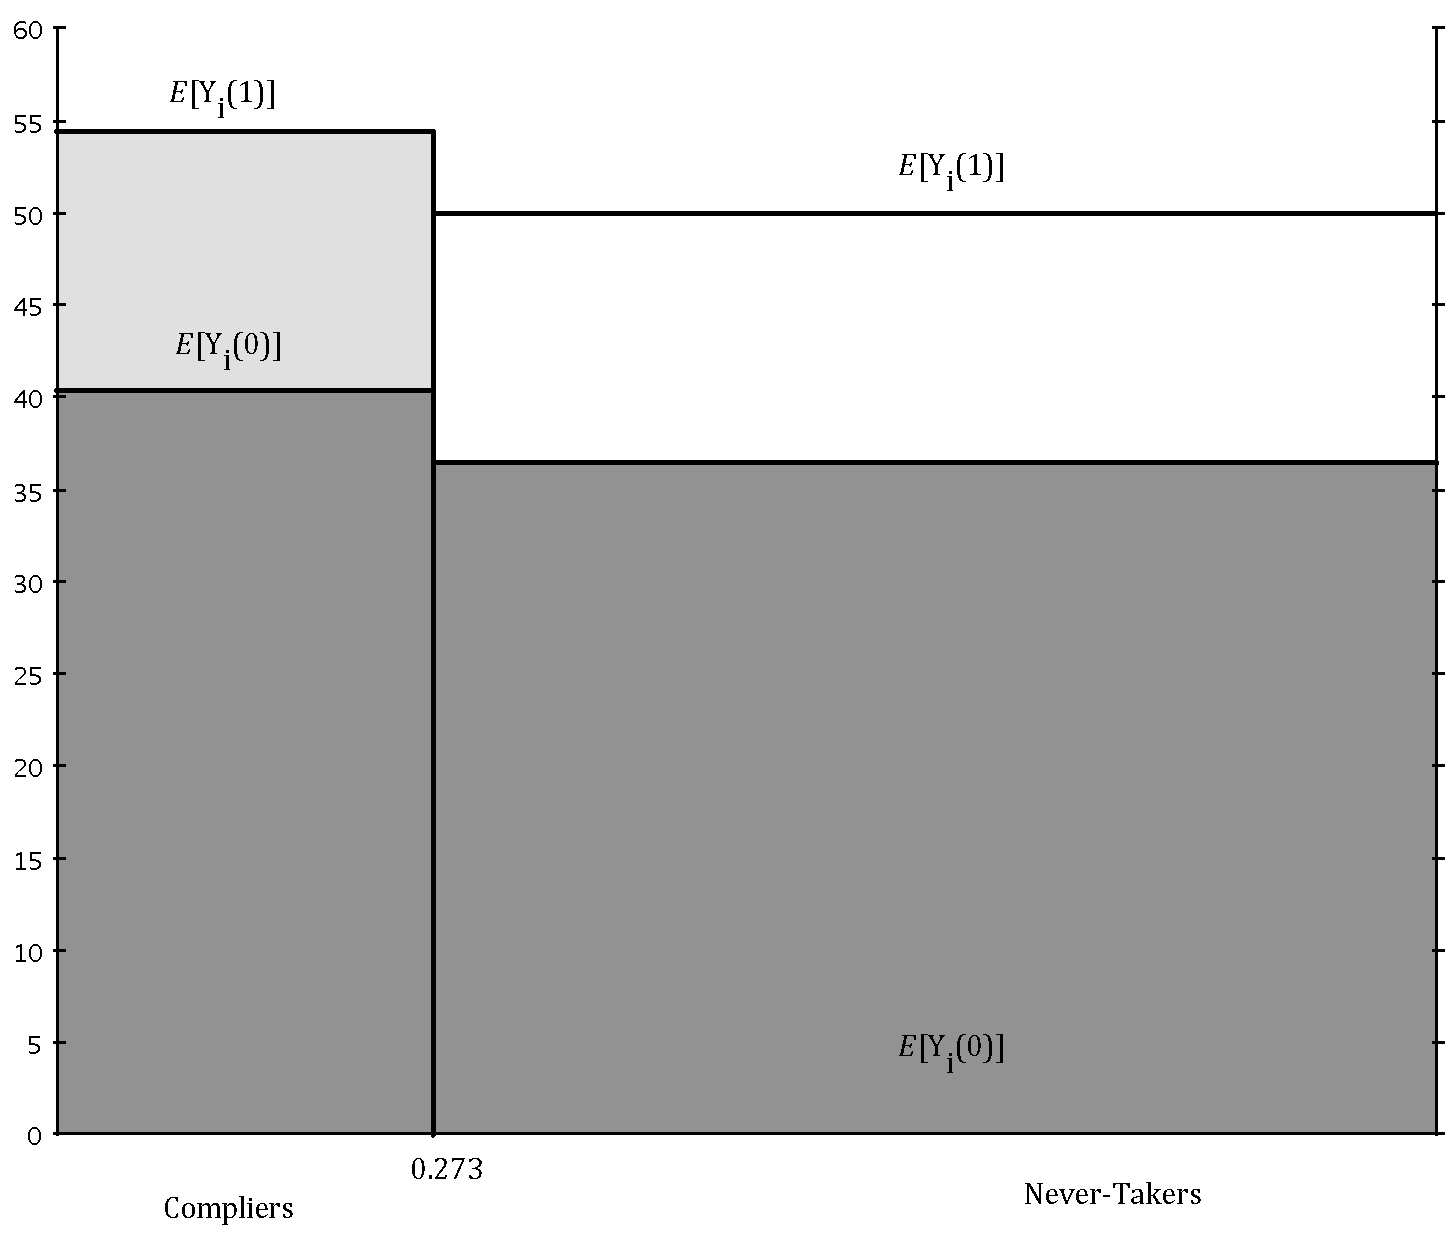
\includegraphics[width=7cm]{../data/Stata_version/figure/PS51btreatment.pdf} }}
    \qquad
    \subfloat[Control Group]{{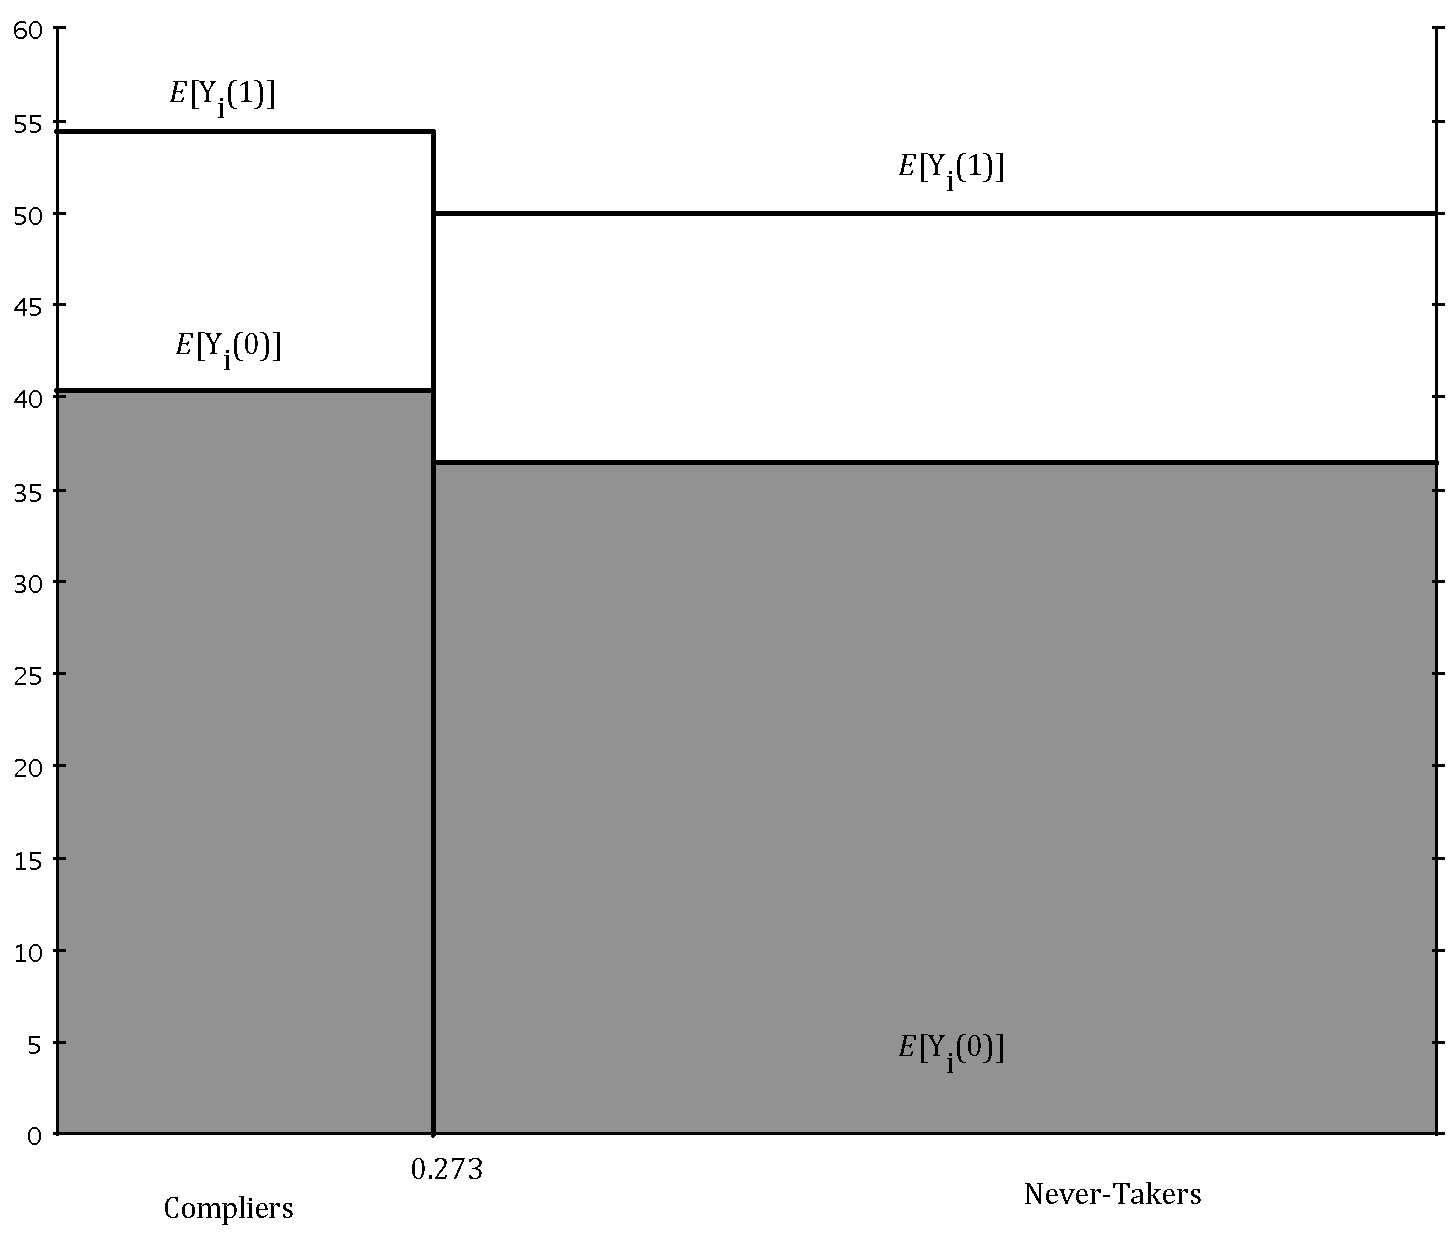
\includegraphics[width=7cm]{../data/Stata_version/figure/PS61bcontrol.pdf} }}
\end{figure}

\end{enumerate}


\section*{Question 2}
Make up a hypothetical schedule of potential outcomes for three Compliers and three Never-Takers in which the ATE is positive but the CACE is negative. Suppose that an experiment were conducted on your pool of subjects. In what ways would the estimated CACE be informative or misleading? [5 pts.]\\
Answer:\\

% Table generated by Excel2LaTeX from sheet 'Sheet1'
\begin{table}[htbp]
  \centering
  \caption{Hypothetical schedule of potential outcomes}
    \begin{tabular}{rrrrrr}
    \toprule
    subject & $Y(0)$  & $Y(1)$  & $D(1)$  & $Y(Z=0)$ & $ Y(Z=1) $\\
    \midrule
    1     & 15    & 5     & 1     & 15    & 5 \\
    2     & 10    & 5     & 1     & 10    & 5 \\
    3     & 5     & 5     & 1     & 5     & 5 \\
    4     & 5     & 25    & 0     & 5     & 5 \\
    5     & 10    & 20    & 0     & 10    & 10 \\
    6     & 15    & 30    & 0     & 15    & 15 \\
    \bottomrule
    \end{tabular}%
  \label{tab:addlabel}%
\end{table}%

\begin{align*}
ATE &= \frac{90 - 60}{6} = 5\\
CACE  &= \frac{15 - 30}{3} = -5
\end{align*}

The estimate of the CACE could be informative if the researcher is interested in what the treatment effect is for those subjects who actually receive the treatment. However, it could be misleading if the researcher attempts to extrapolate these results to the effect of the treatment on the subject pool as a whole, as compliance is a trait revealed post-treatment and could be correlated with potential outcomes such that the conditional treatment affect for compliers is not the same as other latent groups in the subject pool.

\section*{Question 3}
Explain whether each of the following statements is true or false for the case of one-sided noncompliance, assuming that an experiment satisfies non-interference and excludability. [8 pts.]
\begin{enumerate}[a)]
\item If the $ITT$ is negative, the $CACE$ must be negative.\\
Answer:\\
True. The $ITT$ can be written as $E[D(1)]*CACE$. If this quantity is negative, then since $E[D(1)]$ must be non-negative, the $CACE$ must be negative.  
\item The smaller the $ITT_D$, the larger the $CACE$.\\
Answer:\\
False. There is no necessary relationship between the $ITT_D$, the proportion of the subjects that are compliers, and the CACE, the average response of the compliers to the treatment. This confusion sometimes arises due to the algebra of calculating the CACE from the $ITT$ and $ITT_D$. Because the $ITT$ can be written as $ITT_D*CACE$, the $CACE$ can be calculated by $ITT/ITT_D$. From this ratio it might appear that when the $ITT_D$ is smaller we are dividing the ITT by a smaller number, leading to a larger CACE. However, the $ITT$ is a function of the $ITT_D$: the $ITT_D$ is in both the numerator (multiplied by the $CACE$) and the denominator.
\item One cannot identify the CACE if no one in the experiment receives the treatment.\\
Answer:\\
True. If no one receives the treatment, it is impossible to estimate the effect of the treatment. Algebraically, the ITT estimate is divided by zero, leading to an undefined CACE estimate. 
\end{enumerate}

\section*{Question 4}
Explain whether each of the following equalities follows as a consequence of the excludability assumption. [10pts]
\begin{enumerate}[a)]
\item $E[Y_i(z = 1)] = E[Y_i(z = 1) | d_i(1)=1]$ \\
Answer:\\
No. The exclusion restriction (ER) says ignore $Z_i$. However, the ER does not imply that $E[Y(D(1))]$ for the entire subject pool is equal to the average $Y(D(1))$ for the compliers. 
\item $E[Y_i(z = 0,d = 0)| d_i(1) = 0] = E[Y_i(z = 1,d = 0)| d_i(1) =0]$\\
Answer:\\
Yes. According to the ER, $Y(Z=1, D) = Y(Z=0, D)$ for all D.

\item $E[Y_i(z = 1, d(1))] = E[Yi(z = 1), d(0))]$\\
Answer:\\
No. The ER does not imply that $D(1)=D(0)$ for all i.  

\item $E[Y_i(z = 0, d(0))] = E[Yi(z = 1), d(0))]$\\
Answer:\\
Yes. The ER implies that $Y_i(Z=1,D)=Y_i(Z=0,D)$. 
\end{enumerate}
\section*{Question 5}
Critically evaluate the following statement: ``If you are conducting an experiment that encounters one-sided noncompliance, you will never know which of your subjects are Compliers and which of your subjects are Never-Takers.'' [5 pts.]\\
Answer:\\
Subjects are assigned to treatment or control. For those subjects assigned to the control group, all subjects are untreated so there is no way to distinguish among them. For those subject assigned to the treatment group, the Compliers are treated and the Never-Takers are not. This is observable, and so you can tell which subjects are of each type for those assigned to the treatment group. Using the subjects assigned to the treatment group, you can contrast the compliers and never-takers based on pretreatment variables.  However, as suggested by the statement, there is a limit to what you can know about individual subjects assigned to the control group. Since both types remain untreated in the control group, you cannot partition the entire subject pool into compliers and never takers.

\section*{Question 6}
Suppose that a researcher hires a group of canvassers to contact a set of 1,000 voters randomly assigned to a treatment group. When the canvassing effort concludes, the canvassers report that they successfully contacted 500 voters in the treatment group, but the truth is that they only contacted 250. When voter turnout rates are tabulated for the treatment and control groups, it turns out that 400 of the 1,000 subjects in the treatment group voted, as compared to 700 of the 2,000 subjects in the control group (none of whom were contacted). [10 pts.] 
\begin{enumerate}[a)]
\item If you believed that 500 subjects were actually contacted, what would your estimate of the CACE be?\\
Answer:\\
ITT estimate is $0.40 - 0.35 = 0.05$. The $ITT_D$ estimate is = $500/1000 = 0.5$.
\begin{align*}
\widehat{CACE}= \frac{\widehat{ITT}}{\widehat{ITT_D}} = \frac{0.05}{0.5} = 0.10
\end{align*}
\item Suppose you learned that only 250 subjects were actually treated. What would your estimate of the CACE be?\\
Answer:\\
ITT estimate stays the same: $0.40 - 0.35 = 0.05$. The $ITT_D$ estimate is now = $250/1000 = 0.25$.
\begin{align*}
\widehat{CACE}= \frac{\widehat{ITT}}{\widehat{ITT_D}} = \frac{0.05}{0.25} = 0.20
\end{align*}
\item Do the canvassers' exaggerated reports make their efforts seem more or less effective?  When formulating your answer, you may define effectiveness in terms of either the ITT or the CACE.
Answer:\\
The exaggerated reports made their efforts look less effective in terms of the CACE. Since the share of the treatment group that actually received the ``boost'' associated with the treatment was smaller than was claimed, the observed difference was attributed to 500 people being treated rather than 250 being treated. Consequently, the average effect of each treatment seems half as large. There is no effect on the estimate of the number of voters produced by the canvassing effort, which is estimated by the ITT.
\end{enumerate}

\section*{Question 7}
Make up a schedule of potential outcomes that would generate Figure 5.2, which illustrates the consequences of an exclusion restriction violation. Hint: you will need to allow for potential outcomes that respond to both $d$ and $z$. [5 pts.]\\
Answer:\\
Figure 5.2 illustrates a situation in which the potential outcome when untreated among the non-compliers depends on whether the subject is in the treatment versus control group. Note that this is just an example of an exclusion restriction violation, in this case limited to one of the average potential outcomes (untreated non-compliers). Other patterns of ER violations are possible as well.
The 6 quantities needed to construct a figure similar to figure 5.2 are: 
\begin{enumerate}
\item $E[D_i(1)]$
\item $E[(Y(0)|D_i(1) = 0), Z_i = 0]$
\item $E[(Y(0)|D_i(1) = 0), Z_i = 1]$
\item $E[(Y(1)|D_i(1) = 0)]$
\item $E[(Y(0)|D_i(1) = 1)]$
\item $E[(Y(1)|D_i(1) = 1)]$
\end{enumerate}
Further, $E[(Y(0)|D_i(1) = 0), Z_i = 0]$ and $E[(Y(0)|D_i(1) = 0), Z_i = 1]$ must be different -- this is the crucial violation of the exclustion restriction. Suppose the subject pool is comprised of only two type subjects. 25 percent are of type 1 and the remainder are of type 2.

\begin{table}[H]
  \centering
  \caption{Question 7 Table}
    \begin{tabular}{lllll}
    \toprule
    Subject  & $Y(D=1)$ & $Y(D=0, Z=0)$ & $Y(D=0, Z=1)$ & $D(1)$ \\
    \midrule
    Type 1 & 10    & 5     & 5     & 1 \\
    Type 2 & 8     & 4     & 6     & 0 \\
    \bottomrule
    \end{tabular}%
  \label{tab:addlabel}%
\end{table}%

\section*{Question 8}
Cotterill et al. report the results of an experiment conducted in an area of the United Kingdom where only half of the local residents recycle their trash.\footnote{Cotterill et al. 2009.} Canvassers visited homes and encouraged residents to recycle. Outcomes were measured by whether the home put out a recycling bin on at least one occasion during the following three weeks. We restrict our attention here to homes that did not recycle trash during a pre-experimental period of observation. When implementing the intervention, researchers encountered one-sided noncompliance: 1,015 of the 1,849 homes assigned to the treatment group were successfully canvassed; none of the 1,430 homes assigned to the control group were canvassed. These researchers found that 591 homes in the treatment group recycled, as opposed to 377 in the control group. The researchers also observed that 429 of 1,015 homes that were successfully canvassed recycled, as opposed to 539 of the 2,264 homes that were not canvassed. [10 pts.]

\begin{enumerate}[a)]
\item Estimate the $ITT$, and interpret the results.\\
Answer:\\
\begin{align*}
\widehat{ITT} = \frac{591}{1849} - \frac{377}{1430} = 0.32 - 0.264 = .056 
\end{align*}
Assignment to being canvassed caused an estimated 5.6 percentage point increase in recycling.
\item Estimate the $ITT_D$, and interpret the results.
Answer:\\
\begin{align*}
\widehat{ITT_d} = \frac{1015}{1849} = 0.549
\end{align*}
The estimated probability a subject randomly assigned to the treatment group will be canvassed (is a Complier) is 54.9\% 
\item Using the equations in Theorem 5.1 as a guide, write down a model of the expected recycling rate among those assigned to the control group. Do the same for the expected recycling rate among those assigned to the treatment group. Show that under the assumptions of Theorem 5.1, the $CACE$ can be identified based on the design of this experiment.

Answer:\\

Assume that the standard assumptions (Exclusion restriction, non-interference) hold. For each subject, the potential outcomes are a collection of 4 values: $(Y_i(D_i), D_i(Z_i))$. \\

\begin{itemize}
\item Define the $CACE = E[Y_i(1)-Y_i(0)|D_i(1)=1]$.\\
\item Expected value of recycling rate ($Y$) in the control group = \\
$E[Y_i(0)|D_i(1)=1]*ITT_d + E[Y_i(0)|D_i(1)=0]*(1-ITT_d)$\\
\item Expected value of recycling rate in treatment group = \\
$E[Y_i(1)|D_i(1)=1]*ITT_d + E[Y_i(0)|D_i(1)=0]*(1-ITT_d)$\\
\item Expected value of rate of successful canvassing = $E[D_i(1)] = ITT_d$\\
\item Expected value of recycling rate among treatment group minus recycling rate of control group = $[E(Y_i(1)|D_i(1)=1] - E[Y_i(0)|D_i(1)=1)]*(ITT_d) = CACE*ITT_d$.  \\
\item $CACE = [E(Y_i(1)|D_i(1)=1] - E[Y_i(0)|D_i(1)=1)] / (ITT_d)$.\\
\end{itemize}
The expected value of ITT estimate (difference in treatment and control group recycling rates) is equal to the numerator (it is an unbiased estimator), and the expected value of the observed compliance rate is an unbiased estimate of the denominator. The ratio of these estimators is a consistent estimator of $E[Y_i(1)|D_i(1)=1] - E[Y_i(0)|D_i(1)=1)] / (ITT_d)$, therefore the experiment produces enough information to obtain an estimate of the CACE. 

\item Estimate the $CACE$, and interpret the results.\\
Answer:\\

\begin{align*}
\widehat{CACE} = \frac{0.056}{0.549} = 0.102
\end{align*}
 
The estimated average increase in the probability a Complier recycles when treated versus not treated is 10.2 percentage points. 

\item Explain why comparing the recycling rates of the treated and untreated subjects tends to produce misleading estimates of the $CACE$ and $ATE$.\\
Answer:\\
Comparisons of the treated and untreated conflate the effect of the treatment and other differences across the groups that might be correlated with being treated. In contrast to random assignment, which produces groups with the same expected potential outcomes through the procedure, claims about the similarity of the potential outcomes for the actually treated and untreated typically rest on assumptions. In the particular example presented here, an unbiased estimate of the treatment effect for compliers requires an estimate of the average outcome for the compliers when untreated, but the untreated households are a mixture of untreated compliers and non-compliers, rather than a collection of untreated compliers. There is substantial evidence that the average recycling rate among the untreated is lower than the recycling rate among the untreated Compliers. The non-Compliers recycle at a rate of 19.4\%, which is much lower than the control group (a mixture of the two types) recycling rate of 26.4\%. This implies that comparing the treated Compliers with the mixture of untreated Compliers and non-compliers will exaggerate the treatment effect. 
\end{enumerate}

\section*{Question 9}
One way to detect heterogeneous treatment effects across subgroups is to employ a design that randomly manipulates the level of compliance. One such study was conducted in Michigan in 2002.\footnote{Gerber and Green 2005.} Subjects were randomly allocated to three experimental groups. The first treatment group was targeted for a phone call that encouraged subjects to vote in the upcoming November election. The second treatment group was targeted for the same call using the same script on the same day, but more attempts were made to reach subjects. No attempts were made to contact the control group. The table below shows the contact rates and voting rates for each of the three assigned groups. [10 pts.]

\begin{table}[H]
  \centering
  \caption{Question 9 Table}
    \begin{tabular}{rrR{3.5cm}R{3.5cm}}
    \toprule
          & Control  & Treatment group \#1 (minimal effort)  & Treatment group \#2 (maximal effort)  \\
    \midrule
    Percent reached by callers  & 0     & 29.97 & 47.31 \\
    Percent voting  & 55.89 & 55.91 & 56.53 \\
    N     & 317182 & 7500  & 7500 \\
    \bottomrule
    \end{tabular}%
  \label{tab:addlabel}%
\end{table}%

\begin{enumerate}[a)]
\item Define two types of Compliers: those who respond when called with minimal (or maximal) effort and those who respond only when called with maximal effort. Write down a model expressing the expected voting rate among those assigned to the control group as a weighted average of potential outcomes among Minimal Compliers, Maximal Compliers, and Never-Takers. Do the same for the expected rate of voting among those assigned to each of the treatment groups.\\
Answer:\\
Let $Z_i = 0$ (no call), $1$ (minimal effort), or $2$ (maximal effort). $Y_i(Z_i) =1$ if subject $i$ votes, $0$ otherwise. Assuming monotonicity as outlined in the problem description, there are three types ($D_i(0)=0$ for all types): 
\begin{itemize}
\item $D_i(1) = D_i(2) = 0$   [Never-Takers]
\item $D_i(2) = 1, D_i(1)=1$	[Easy to reach subjects, or Minimal Effort Compliers]
\item $D_i(2) = 1, D_i(1) = 0$	[Hard to reach subjects, or Maximal Effort Compliers]
\end{itemize}

\begin{align*}
\text{Expected Vote rate in Control (EV, Control)} &= \\
&E(Y(0)|\text{ never taker})*Pr(\text{never taker}) + \\
&E(Y(0)|\text{ easy to reach})*Pr(\text{easy to reach}) + \\
&E(Y(0)|\text{ hard to reach})*Pr(\text{hard to reach})
\end{align*}

\begin{align*}
\text{Expected Vote rate in minimal effort (EV, minimal)} &= \\
&E(Y(0)|\text{ never taker})*Pr(\text{never taker}) + \\
&E(Y(1)|\text{ easy to reach})*Pr(\text{easy to reach}) + \\
&E(Y(0)|\text{ hard to reach})*Pr(\text{hard to reach})
\end{align*}

\begin{align*}
\text{Expected Vote rate in maximal effort (EV, maximal)} &= \\
&E(Y(0)|\text{ never taker})*Pr(\text{never taker}) + \\
&E(Y(1)|\text{ easy to reach})*Pr(\text{easy to reach}) + \\
&E(Y(1)|\text{ hard to reach})*Pr(\text{hard to reach})
\end{align*}


\item Show that the CACE for each of the treatments can be identified based on the design of this experiment.

\begin{align*}
\text{(EV, minimal - EV,control)} &= \\
&E(Y(1)|\text{ easy to reach})*Pr(\text{easy to reach}) - \\
&E(Y(0)|\text{ easy to reach})*Pr(\text{easy to reach}) \\
&= E(Y(1) -(Y(0)|\text{ easy to reach})*Pr(\text{easy to reach}) \\
&= (\text{ATE}|\text{ easy to reach})*Pr(\text{easy to reach}). \\
\text{ATE|\text{ easy to reach}} &= \frac{\text{(EV, minimal - EV,control)}}{Pr(\text{easy to reach})}
\end{align*}

Similarly, 
\begin{align*}
\text{(EV, maximal - EV,minimal)} &= \\
&E(Y(1)|\text{ hard to reach})*Pr(\text{hard to reach}) - \\
&E(Y(0)|\text{ hard to reach})*Pr(\text{hard to reach}) \\
&= E(Y(1) -(Y(0)|\text{ hard to reach})*Pr(\text{hard to reach}) \\
&= (\text{ATE}|\text{ hard to reach})*Pr(\text{hard to reach}). \\
\text{ATE|\text{ hard to reach}} &= \frac{\text{(EV, maximal - EV,minimal)}}{Pr(\text{hard to reach})}
\end{align*}

To estimate the numerators, which involve EV for the subject pool when untreated, given the minimal treatment or maximal treatment, use the average of the randomly assigned groups, which are unbiased estimators of the respective quantities.
To obtain unbiased estimates of the subject pool proportions for the three types, the proportion that complies in the minimal treatment group is an unbiased estimate of the proportion of easy to reach, and the proportion that complies in the maximal effort group is an estimate of the combined proportion of easy and hard to reach. Subtract the estimated proportion that is easy to reach to obtain the proportion that is hard to reach.


\item Estimate the share of the subject pool that Maximal Compliers comprise. Estimate the share of the subject pool that Minimal Compliers comprise.\\
Answer:\\
The share of compliers in the minimal treatment group provides an estimate of the share of easy to reach: 29.97\% \\
The share of compliers in the maximal treatment group provides an estimate of the share of easy to reach plus the share of hard to reach, which equals 47.31. Subtracting the estimated share of the easy to reach, 29.97\%, produces an estimate of the share of hard to reach, 47.31 - 29.97 = 17.34\%. 

\item Estimate the average treatment effect among each type of Complier, and interpret the results.
Answer:\\
The CACE for the easy to reach: $\frac{0.5591 - 0.5589}{0.2997} = 0.0007$ \\ 
The CACE for the hard to reach: $\frac{0.5653 - 0.5591}{0.1734} = 0.0358$ \\
The treatment effect estimate for the hard to reach is larger than the estimated effect for the easy to reach, although further calculations are needed to determine whether the difference in CACEs is greater than one would expect from random sampling variability.

\end{enumerate}

\section*{Question 10}
Guan and Green report the results of a canvassing experiment conducted in Beijing on the eve of a local election.\footnote{Guan and Green 2006.} Students on the campus of Peking University were randomly assigned to treatment or control groups. Canvassers attempted to contact students in their dorm rooms and encourage them to vote. No contact with the control group was attempted. Of the 2,688 students assigned to the treatment group, 2,380 were contacted. A total of 2,152 students in the treatment group voted; of the 1,334 students assigned to the control group, 892 voted. One aspect of this experiment threatens to violate the exclusion restriction. At every dorm room they visited, even those where no one answered, canvassers left a leaflet encouraging students to vote. [12 pts.]



\begin{enumerate}[a)]
\item Using the dataset at http://isps.research.yale.edu/FEDAI, estimate the $ITT$.
\begin{knitrout}
\definecolor{shadecolor}{rgb}{0.969, 0.969, 0.969}\color{fgcolor}\begin{kframe}
\begin{Verbatim}[commandchars=\\\{\}]
{\color{incolor}In [{\color{incolor}1}]:} \PY{k}{set}\PY{k}{ more} off
        \PY{k}{qui} import delim .\PY{o}{/}data\PY{o}{/}chapter05\PY{o}{/}Guan\PYZus{}Green\PYZus{}CPS\PYZus{}2006,\PY{k}{ clear}
\end{Verbatim}
    \begin{Verbatim}[commandchars=\\\{\}]
{\color{incolor}In [{\color{incolor}2}]:} \PY{k}{qui}\PY{k}{ drop}\PY{k}{ if} turnout \PY{o}{==} .
        \PY{k}{qui}\PY{k}{ drop}\PY{k}{ if} contact \PY{o}{==} .
        \PY{k}{qui}\PY{k}{ drop}\PY{k}{ if} dormid \PY{o}{==} .
        \PY{k}{qui}\PY{k}{ drop}\PY{k}{ if} treat2 \PY{o}{==} . 
        
        \PY{k}{rename} treat2 Z
        \PY{k}{rename} turnout Y
        \PY{k}{rename} contact D
        \PY{k}{rename} dormid clust
\end{Verbatim}

    \begin{Verbatim}[commandchars=\\\{\}]
{\color{incolor}In [{\color{incolor}3}]:} \PY{k}{tabstat} Y,\PY{k}{ by}(Z) stat(mean)\PY{k}{ save}
        \PY{c+c1}{//}\PY{c+c1}{ }\PY{c+c1}{I}\PY{c+c1}{T}\PY{c+c1}{T}
        \PY{k}{di} \PY{n+nFormat}{\PYZpc{}8.7f} \PY{n+nf}{el}(\PY{n+nf}{r}(Stat2),\PY{l+m}{1} ,\PY{l+m}{1}) \PY{o}{\PYZhy{}} \PY{n+nf}{el}(\PY{n+nf}{r}(Stat1),\PY{l+m}{1} ,\PY{l+m}{1})
\end{Verbatim}

    \begin{Verbatim}[commandchars=\\\{\}]
Summary for variables: Y
     by categories of: Z 

       Z |      mean
---------+----------
       0 |  .6686657
       1 |  .8005952
---------+----------
   Total |  .7568374
--------------------

0.1319296

    \end{Verbatim}

\end{kframe}
\end{knitrout}

The estimated ITT is 0.132.

\item Use randomization inference to test the sharp null hypothesis that the $ITT$ is zero for all observations, taking into account the fact that random assignment was clustered by dorm room. Interpret your results.
\begin{knitrout}
\definecolor{shadecolor}{rgb}{0.969, 0.969, 0.969}\color{fgcolor}\begin{kframe}
   \begin{Verbatim}[commandchars=\\\{\}]
{\color{incolor}In [{\color{incolor}4}]:} \PY{k}{preserve}
        \PY{k}{collapse} Z,\PY{k}{ by}(clust)   
        \PY{k}{qui}\PY{k}{ sum} Z
        \PY{k}{global} p = \PY{n+nf}{r}(mean)
        \PY{k}{restore}
\end{Verbatim}

    \begin{Verbatim}[commandchars=\\\{\}]
{\color{incolor}In [{\color{incolor}5}]:} \PY{c+c1}{//}\PY{c+c1}{ }\PY{c+c1}{p}\PY{c+c1}{r}\PY{c+c1}{o}\PY{c+c1}{b}\PY{c+c1}{a}\PY{c+c1}{b}\PY{c+c1}{i}\PY{c+c1}{l}\PY{c+c1}{i}\PY{c+c1}{t}\PY{c+c1}{y}\PY{c+c1}{ }\PY{c+c1}{o}\PY{c+c1}{f}\PY{c+c1}{ }\PY{c+c1}{b}\PY{c+c1}{e}\PY{c+c1}{i}\PY{c+c1}{n}\PY{c+c1}{g}\PY{c+c1}{ }\PY{c+c1}{a}\PY{c+c1}{s}\PY{c+c1}{s}\PY{c+c1}{i}\PY{c+c1}{g}\PY{c+c1}{n}\PY{c+c1}{e}\PY{c+c1}{d}\PY{c+c1}{ }\PY{c+c1}{t}\PY{c+c1}{o}\PY{c+c1}{ }\PY{c+c1}{t}\PY{c+c1}{r}\PY{c+c1}{e}\PY{c+c1}{a}\PY{c+c1}{t}\PY{c+c1}{m}\PY{c+c1}{e}\PY{c+c1}{n}\PY{c+c1}{t}
        \PY{k}{gen} probs = \PY{n+nv+vg}{\PYZdl{}}\PY{n+nv+vg}{p}
        
        
        ritest Z \PYZus{}b[Z],\PY{k}{ cluster}(clust) reps(\PY{l+m}{10000}) nodots: \PY{c+cs}{///}
        \PY{k}{regress} Y Z
\end{Verbatim}

    \begin{Verbatim}[commandchars=\\\{\}]
  res. var(s):  Z
   Resampling:  Permuting Z
Clust. var(s):  clust
     Clusters:  1004
Strata var(s):  none
       Strata:  1

------------------------------------------------------------------------------
T            |     T(obs)       c       n   p=c/n   SE(p) [95\% Conf. Interval]
-------------+----------------------------------------------------------------
       \_pm\_1 |   .1319296       0   10000  0.0000  0.0000         0   .0003688
------------------------------------------------------------------------------
Note: Confidence interval is with respect to p=c/n.
Note: c = \#\{|T| >= |T(obs)|\}

    \end{Verbatim}

    \begin{Verbatim}[commandchars=\\\{\}]
{\color{incolor}In [{\color{incolor}6}]:} \PY{c+c1}{//}\PY{c+c1}{ }\PY{c+c1}{i}\PY{c+c1}{t}\PY{c+c1}{t}
        \PY{k}{di} \PY{n+nFormat}{\PYZpc{}8.4f} \PY{n+nf}{el}(\PY{n+nf}{r}(b),\PY{l+m}{1},\PY{l+m}{1})
\end{Verbatim}

    \begin{Verbatim}[commandchars=\\\{\}]
  0.1319

    \end{Verbatim}

    \begin{Verbatim}[commandchars=\\\{\}]
{\color{incolor}In [{\color{incolor}7}]:} \PY{c+c1}{//}\PY{c+c1}{ }\PY{c+c1}{p}\PY{c+c1}{.}\PY{c+c1}{v}\PY{c+c1}{a}\PY{c+c1}{l}\PY{c+c1}{u}\PY{c+c1}{e}\PY{c+c1}{.}\PY{c+c1}{t}\PY{c+c1}{w}\PY{c+c1}{o}\PY{c+c1}{s}\PY{c+c1}{i}\PY{c+c1}{d}\PY{c+c1}{e}\PY{c+c1}{d}
        \PY{k}{di} \PY{n+nFormat}{\PYZpc{}8.0f} \PY{n+nf}{el}(\PY{n+nf}{r}(p),\PY{l+m}{1},\PY{l+m}{1})
\end{Verbatim}

    \begin{Verbatim}[commandchars=\\\{\}]
       0
    \end{Verbatim}
\end{kframe}
\end{knitrout}

\item Assume that the leaflet had no effect on turnout. Estimate the $CACE$.
\begin{knitrout}
\definecolor{shadecolor}{rgb}{0.969, 0.969, 0.969}\color{fgcolor}\begin{kframe}
    \begin{Verbatim}[commandchars=\\\{\}]
{\color{incolor}In [{\color{incolor}8}]:} \PY{k}{qui}\PY{k}{ regress} Y Z
        \PY{k}{scalar} itt = \PYZus{}b[Z]
        \PY{k}{di} \PY{n+nFormat}{\PYZpc{}8.4f} itt
\end{Verbatim}

    \begin{Verbatim}[commandchars=\\\{\}]
  0.1319
    \end{Verbatim}

    \begin{Verbatim}[commandchars=\\\{\}]
{\color{incolor}In [{\color{incolor}9}]:} \PY{k}{qui}\PY{k}{ regress} D Z
        \PY{k}{scalar} ittd = \PYZus{}b[Z]
        \PY{k}{di} \PY{n+nFormat}{\PYZpc{}8.4f} ittd
\end{Verbatim}

    \begin{Verbatim}[commandchars=\\\{\}]
  0.8858
    \end{Verbatim}

    \begin{Verbatim}[commandchars=\\\{\}]
{\color{incolor}In [{\color{incolor}10}]:} \PY{k}{scalar} cace = itt\PY{o}{/}ittd
         \PY{k}{di} \PY{n+nFormat}{\PYZpc{}8.4f} cace
\end{Verbatim}

    \begin{Verbatim}[commandchars=\\\{\}]
  0.1489
    \end{Verbatim}
\end{kframe}
\end{knitrout}
\item Assume that the leaflet raised the probability of voting by one percentage point among both Compliers and Never-Takers. In other words, suppose that the treatment group's turnout rate would have been one percentage point lower had the leaflets not been distributed. Write down a model of the expected turnout rates in the treatment and control groups, incorporating the average effect of the leaflet.\\
Answer:\\
Let $Y_i(1)$ be whether $i$ votes when reached for canvassing but not treated with a leaflet, $Y_i(0)$ be whether $i$ votes when not reached for canvassing and not left a leaflet. Let $D_i = 1$ when canvassed when assigned to treatment group, 0 otherwise.\\
Expected Turnout in Treatment Group (EV, Treatment):
\begin{align*}
& E[Y_i(1) + .01)|d_i(1)=1]*ITT_d + E[Y_i(0)+.01)|d_i(1)=0]*(1-ITT_d) = \\
& E[Y_i(1)|d_i(1)=1]*ITT_d + E[Y_i(0)|d_i(1)=0]*(1-ITT_d) + .01\\
\end{align*}
Expected Turnout in Control Group (EV, Control):
\begin{align*}
& E[Y_i(0)|d_i(1)=1]*ITT_d + E[Y_i(0)|d_i(1)=0]*(1-ITT_d) \\
\end{align*}
(EV, Treatment) - (EV, Control) = ITT:
\begin{align*}
ITT &= .01 + E[Y_i(1)|d_i(1)=1]*ITT_d  - E[Y_i(0)|d_i(1)=1]*ITT_d\\
&= .01 + E[Y_i(1) - Y_i(0)|d_i(1)=1]*ITT_d \\
ITT/ITTd &=  E[Y_i(1) - Y_i(0)|d_i(1)=1] + \frac{.01}{ITT_d}.\\ 
\end{align*}
Therefore:
\begin{align*}
CACE &= E (Yi(1) - Yi(0)|di(1)=1) = ITT/ITTd - .01/ITTd
\end{align*}

\item Given this assumption, estimate the CACE of canvassing.
\begin{align*}
\widehat{CACE} = 0.149 - \frac{0.01}{0.885} = 0.138
\end{align*}
\item Suppose, instead, that the leaflet had no effect on Compliers (who heard the canvasser's speech and ignored the leaflet) but raised turnout among Never-Takers by 3 percentage points. Given this assumption, estimate the CACE of canvassing.\\
Answer:\\
Under this assumption, we write:\\
Expected Turnout in Treatment Group (EV, Treatment)=
\begin{align*}
E[Y_i(1)|d_i(1)=1]* ITT_d + E[Y_i(0)+.03)|d_i(1)=0]*(1-ITT_d)
\end{align*}
Therefore, subtracting the expected vote in the control group from the expected vote in the treatment group gives:

\begin{align*}
ITT &= E[Y_i(1)|d_i(1)=1]* ITT_d + E[Y_i(0)+.03)|d_i(1)=0]*(1-ITT_d) - \\
& E[Y_i(0)|d_i(1)=1]*ITT_d - E[Y_i(0)|d_i(1)=0]*(1-ITT_d) \\
&= E[Y_i(1) - Y_i(0)|d_i(1)=1]*ITT_d + 0.03*(1-ITT_d)
\end{align*}

Therefore:
\begin{align*}
\frac{ITT}{ITT_d} &= CACE + \frac{0.03(1-ITT_d)}{ITT_d}\\
CACE &= \frac{ITT}{ITT_d} - \frac{0.03(1-ITT_d)}{ITT_d}\\
&= \frac{0.132}{0.885} - \frac{0.03(1-0.885)}{0.885}\\
&= 0.145
\end{align*}



\end{enumerate}

\section*{Question 11}
Nickerson describes a voter mobilization experiment in which subjects were randomly assigned to one of three conditions: a baseline group (no contact was attempted), a treatment group (canvassers attempted to deliver an encouragement to vote), and a placebo group (canvassers attempted to deliver an encouragement to recycle).\footnote{Nickerson 2005, 2008.} Based on the results presented below, calculate the following: [10 pts.]
% Table generated by Excel2LaTeX from sheet 'Sheet1'
\begin{table}[H]
  \centering
  \caption{Question 11 Table}
    \begin{tabular}{rrrr}
    \toprule
    Treatment assignment  & Treated?  & N     & Turnout  \\
    \midrule
    \multicolumn{1}{c}{Baseline}  & No    & 2572  & 0.3122 \\
    \multicolumn{1}{c}{\multirow{2}[0]{*}{Treatment }} & Yes   & 486   & 0.3909 \\
    \multicolumn{1}{c}{} & No    & 2086  & 0.3274 \\
    \multicolumn{1}{c}{\multirow{2}[0]{*}{Placebo }} & Yes   & 470   & 0.2979 \\
    \multicolumn{1}{c}{} & No    & 2109  & 0.3215 \\
    \bottomrule
    \end{tabular}%
  \label{tab:addlabel}%
\end{table}%

\begin{enumerate}[a)]
\item Estimate the proportion of Compliers based on subjects' responses to the treatment.
Estimate the proportion of Compliers based on subjects' responses to the placebo. Assuming that the individuals are assigned randomly to the treatment and placebo groups, are these rates of compliance consistent with the null hypothesis that both groups have the same proportion of Compliers? \\

\begin{knitrout}
\definecolor{shadecolor}{rgb}{0.969, 0.969, 0.969}\color{fgcolor}\begin{kframe}
   \begin{Verbatim}[commandchars=\\\{\}]
{\color{incolor}In [{\color{incolor}1}]:} \PY{k}{clear}
        \PY{k}{qui}\PY{k}{ set} obs \PY{l+m}{7723}
        \PY{c+c1}{//}\PY{c+c1}{ }\PY{c+c1}{s}\PY{c+c1}{s}\PY{c+c1}{c}\PY{c+c1}{ }\PY{c+c1}{i}\PY{c+c1}{n}\PY{c+c1}{s}\PY{c+c1}{t}\PY{c+c1}{a}\PY{c+c1}{l}\PY{c+c1}{l}\PY{c+c1}{ }\PY{c+c1}{e}\PY{c+c1}{g}\PY{c+c1}{e}\PY{c+c1}{n}\PY{c+c1}{m}\PY{c+c1}{o}\PY{c+c1}{r}\PY{c+c1}{e}\PY{c+c1}{ }\PY{c+c1}{(}\PY{c+c1}{i}\PY{c+c1}{n}\PY{c+c1}{s}\PY{c+c1}{t}\PY{c+c1}{a}\PY{c+c1}{l}\PY{c+c1}{l}\PY{c+c1}{ }\PY{c+c1}{t}\PY{c+c1}{h}\PY{c+c1}{e}\PY{c+c1}{ }\PY{c+c1}{p}\PY{c+c1}{a}\PY{c+c1}{c}\PY{c+c1}{k}\PY{c+c1}{a}\PY{c+c1}{g}\PY{c+c1}{e}\PY{c+c1}{)}
        \PY{k}{qui}\PY{k}{ egen} z =\PY{k}{ repeat}(), values(\PY{l+s}{\PYZdq{}}\PY{l+s}{b}\PY{l+s}{a}\PY{l+s}{s}\PY{l+s}{e}\PY{l+s}{l}\PY{l+s}{i}\PY{l+s}{n}\PY{l+s}{e}\PY{l+s}{\PYZdq{}})
        \PY{k}{qui}\PY{k}{ replace} z = \PY{l+s}{\PYZdq{}}\PY{l+s}{t}\PY{l+s}{r}\PY{l+s}{e}\PY{l+s}{a}\PY{l+s}{t}\PY{l+s}{m}\PY{l+s}{e}\PY{l+s}{n}\PY{l+s}{t}\PY{l+s}{\PYZdq{}}\PY{k}{ in} \PY{l+m}{2573}\PY{o}{/}\PY{l+m}{5144}
        \PY{k}{qui}\PY{k}{ replace} z = \PY{l+s}{\PYZdq{}}\PY{l+s}{p}\PY{l+s}{l}\PY{l+s}{a}\PY{l+s}{c}\PY{l+s}{e}\PY{l+s}{b}\PY{l+s}{o}\PY{l+s}{\PYZdq{}}\PY{k}{ in} \PY{l+m}{5145}\PY{o}{/}\PY{l+m}{7723}
        \PY{k}{qui}\PY{k}{ egen}\PY{k}{ d} = fill(\PY{l+m}{0},\PY{l+m}{0})
        \PY{k}{qui}\PY{k}{ replace}\PY{k}{ d} = \PY{l+m}{1}\PY{k}{ in} \PY{l+m}{2573}\PY{o}{/}\PY{l+m}{3058}
        \PY{k}{qui}\PY{k}{ replace}\PY{k}{ d} = \PY{l+m}{1}\PY{k}{ in} \PY{l+m}{5145}\PY{o}{/}\PY{l+m}{5614}
        \PY{k}{qui}\PY{k}{ egen} y = fill(\PY{l+m}{1},\PY{l+m}{1})
        \PY{k}{qui}\PY{k}{ replace} y=\PY{l+m}{0}\PY{k}{ in} \PY{l+m}{804}\PY{o}{/}\PY{l+m}{2572}
        \PY{k}{qui}\PY{k}{ replace} y=\PY{l+m}{0}\PY{k}{ in} \PY{l+m}{2763}\PY{o}{/}\PY{l+m}{3058}
        \PY{k}{qui}\PY{k}{ replace} y=\PY{l+m}{0}\PY{k}{ in} \PY{l+m}{3742}\PY{o}{/}\PY{l+m}{5144}
        \PY{k}{qui}\PY{k}{ replace} y=\PY{l+m}{0}\PY{k}{ in} \PY{l+m}{5285}\PY{o}{/}\PY{l+m}{5614}
        \PY{k}{qui}\PY{k}{ replace} y=\PY{l+m}{0}\PY{k}{ in} \PY{l+m}{6293}\PY{o}{/}\PY{l+m}{7723}
\end{Verbatim}

    \begin{Verbatim}[commandchars=\\\{\}]
{\color{incolor}In [{\color{incolor}2}]:} \PY{k}{qui}\PY{k}{ sum}\PY{k}{ d}\PY{k}{ if} z\PY{o}{==}\PY{l+s}{\PYZdq{}}\PY{l+s}{t}\PY{l+s}{r}\PY{l+s}{e}\PY{l+s}{a}\PY{l+s}{t}\PY{l+s}{m}\PY{l+s}{e}\PY{l+s}{n}\PY{l+s}{t}\PY{l+s}{\PYZdq{}}
        \PY{k}{scalar} pr\PYZus{}c\PYZus{}treatment =  \PY{n+nf}{r}(mean)
        \PY{k}{di} \PY{n+nFormat}{\PYZpc{}8.3f} pr\PYZus{}c\PYZus{}treatment
\end{Verbatim}

    \begin{Verbatim}[commandchars=\\\{\}]
   0.189
    \end{Verbatim}

    \begin{Verbatim}[commandchars=\\\{\}]
{\color{incolor}In [{\color{incolor}3}]:} \PY{k}{qui}\PY{k}{ sum}\PY{k}{ d}\PY{k}{ if} z\PY{o}{==}\PY{l+s}{\PYZdq{}}\PY{l+s}{p}\PY{l+s}{l}\PY{l+s}{a}\PY{l+s}{c}\PY{l+s}{e}\PY{l+s}{b}\PY{l+s}{o}\PY{l+s}{\PYZdq{}}
        \PY{k}{scalar} pr\PYZus{}c\PYZus{}placebo =  \PY{n+nf}{r}(mean)
        \PY{k}{di} \PY{n+nFormat}{\PYZpc{}8.4f} pr\PYZus{}c\PYZus{}placebo
\end{Verbatim}

    \begin{Verbatim}[commandchars=\\\{\}]
  0.1822
    \end{Verbatim}
\end{kframe}
\end{knitrout}

The estimated proportion of compliers in the vote encouragement group is 0.189. The estimated proportion in the placebo group is 0.182. The difference between these rates is fairly small and not statistically significant. These rates of compliance are consistent with the null hypothesis that both groups have the same proportion of Compliers.

\item Do the data suggest that Never-Takers in the treatment and placebo groups have the same rate of turnout? Is this comparison informative?\\
\begin{knitrout}
\definecolor{shadecolor}{rgb}{0.969, 0.969, 0.969}\color{fgcolor}\begin{kframe}
   \begin{Verbatim}[commandchars=\\\{\}]
{\color{incolor}In [{\color{incolor}4}]:} \PY{c+c1}{//}\PY{c+c1}{ }\PY{c+c1}{r}\PY{c+c1}{a}\PY{c+c1}{t}\PY{c+c1}{e}\PY{c+c1}{.}\PY{c+c1}{n}\PY{c+c1}{t}\PY{c+c1}{.}\PY{c+c1}{t}\PY{c+c1}{r}\PY{c+c1}{e}\PY{c+c1}{a}\PY{c+c1}{t}\PY{c+c1}{m}\PY{c+c1}{e}\PY{c+c1}{n}\PY{c+c1}{t}
        \PY{k}{qui}\PY{k}{ sum} y\PY{k}{ if} z\PY{o}{==}\PY{l+s}{\PYZdq{}}\PY{l+s}{t}\PY{l+s}{r}\PY{l+s}{e}\PY{l+s}{a}\PY{l+s}{t}\PY{l+s}{m}\PY{l+s}{e}\PY{l+s}{n}\PY{l+s}{t}\PY{l+s}{\PYZdq{}} \PY{o}{\PYZam{}}\PY{k}{ d}\PY{o}{==}\PY{l+m}{0} 
        \PY{k}{di} \PY{n+nFormat}{\PYZpc{}8.4f} \PY{n+nf}{r}(mean)
\end{Verbatim}

    \begin{Verbatim}[commandchars=\\\{\}]
  0.3274
    \end{Verbatim}

    \begin{Verbatim}[commandchars=\\\{\}]
{\color{incolor}In [{\color{incolor}5}]:} \PY{c+c1}{//}\PY{c+c1}{ }\PY{c+c1}{r}\PY{c+c1}{a}\PY{c+c1}{t}\PY{c+c1}{e}\PY{c+c1}{.}\PY{c+c1}{n}\PY{c+c1}{t}\PY{c+c1}{.}\PY{c+c1}{p}\PY{c+c1}{l}\PY{c+c1}{a}\PY{c+c1}{c}\PY{c+c1}{e}\PY{c+c1}{b}\PY{c+c1}{o}
        \PY{k}{qui}\PY{k}{ sum} y\PY{k}{ if} z\PY{o}{==}\PY{l+s}{\PYZdq{}}\PY{l+s}{p}\PY{l+s}{l}\PY{l+s}{a}\PY{l+s}{c}\PY{l+s}{e}\PY{l+s}{b}\PY{l+s}{o}\PY{l+s}{\PYZdq{}} \PY{o}{\PYZam{}}\PY{k}{ d}\PY{o}{==}\PY{l+m}{0}
        \PY{k}{di} \PY{n+nFormat}{\PYZpc{}8.4f} \PY{n+nf}{r}(mean)
\end{Verbatim}

    \begin{Verbatim}[commandchars=\\\{\}]
  0.3215
    \end{Verbatim}
\end{kframe}
\end{knitrout}
Yes, the turnout rate among the encouragement never takers is 32.7\% versus 32.2\% for the placebo group. If $D_i(1)$ is the same for all subjects whether the $Z=1$ means that they are assigned to the placebo or the encouragement, and the subjects are randomly assigned to each group, then the groups of untreated placebo and encouragement subjects are formed by random assignment from the same pool of subjects (the non-compliers). A prediction that follows from this claim is that placebo and the encouragement groups have the same expected average potential outcomes when untreated. If the observed difference in average potential outcomes when untreated is too large, we may reject the maintained hypothesis that the group is formed by random draws from a common pool of subjects. One implication of this is that perhaps the pattern of subject compliance is not the same for the two treatments.

\item Estimate the CACE of receiving the placebo. Is this estimate consistent with the substantive assumption that the placebo has no effect on turnout?\\
\begin{knitrout}
\definecolor{shadecolor}{rgb}{0.969, 0.969, 0.969}\color{fgcolor}\begin{kframe}
   \begin{Verbatim}[commandchars=\\\{\}]
{\color{incolor}In [{\color{incolor}6}]:} \PY{k}{qui}\PY{k}{ sum} y\PY{k}{ if} z\PY{o}{==}\PY{l+s}{\PYZdq{}}\PY{l+s}{p}\PY{l+s}{l}\PY{l+s}{a}\PY{l+s}{c}\PY{l+s}{e}\PY{l+s}{b}\PY{l+s}{o}\PY{l+s}{\PYZdq{}}
        \PY{k}{scalar} y\PYZus{}placebo = \PY{n+nf}{r}(mean)
        \PY{k}{qui}\PY{k}{ sum} y\PY{k}{ if} z\PY{o}{==}\PY{l+s}{\PYZdq{}}\PY{l+s}{b}\PY{l+s}{a}\PY{l+s}{s}\PY{l+s}{e}\PY{l+s}{l}\PY{l+s}{i}\PY{l+s}{n}\PY{l+s}{e}\PY{l+s}{\PYZdq{}}
        \PY{k}{scalar} y\PYZus{}baseline = \PY{n+nf}{r}(mean)
\end{Verbatim}

    \begin{Verbatim}[commandchars=\\\{\}]
{\color{incolor}In [{\color{incolor}7}]:} \PY{k}{scalar} itt\PYZus{}placebo = y\PYZus{}placebo \PY{o}{\PYZhy{}} y\PYZus{}baseline
        \PY{k}{scalar} cace\PYZus{}placebo = itt\PYZus{}placebo\PY{o}{/}pr\PYZus{}c\PYZus{}placebo
\end{Verbatim}

    \begin{Verbatim}[commandchars=\\\{\}]
{\color{incolor}In [{\color{incolor}8}]:} \PY{c+c1}{//}\PY{c+c1}{ }\PY{c+c1}{E}\PY{c+c1}{s}\PY{c+c1}{t}\PY{c+c1}{i}\PY{c+c1}{m}\PY{c+c1}{a}\PY{c+c1}{t}\PY{c+c1}{e}\PY{c+c1}{ }\PY{c+c1}{t}\PY{c+c1}{h}\PY{c+c1}{e}\PY{c+c1}{ }\PY{c+c1}{C}\PY{c+c1}{A}\PY{c+c1}{C}\PY{c+c1}{E}\PY{c+c1}{ }\PY{c+c1}{o}\PY{c+c1}{f}\PY{c+c1}{ }\PY{c+c1}{r}\PY{c+c1}{e}\PY{c+c1}{c}\PY{c+c1}{e}\PY{c+c1}{i}\PY{c+c1}{v}\PY{c+c1}{i}\PY{c+c1}{n}\PY{c+c1}{g}\PY{c+c1}{ }\PY{c+c1}{t}\PY{c+c1}{h}\PY{c+c1}{e}\PY{c+c1}{ }\PY{c+c1}{p}\PY{c+c1}{l}\PY{c+c1}{a}\PY{c+c1}{c}\PY{c+c1}{e}\PY{c+c1}{b}\PY{c+c1}{o}
        \PY{k}{disp} \PY{n+nFormat}{\PYZpc{}8.3f} cace\PYZus{}placebo
\end{Verbatim}

    \begin{Verbatim}[commandchars=\\\{\}]
   0.027
    \end{Verbatim}

\end{kframe}
\end{knitrout}

The CACE is 0.027. The placebo has an unexpectedly positive effect on turnout (although further analysis shows that the effect is not larger than one would expect due to random sampling variability). The fact that the placebo group has higher turnout than the control group makes the GOTV vs. placebo comparison more conservative.

\item Estimate the CACE of receiving the treatment using two different methods. First, use the conventional method of dividing the $ITT$ by the $ITT_D$. Second, compare turnout rates among Compliers in both the treatment and placebo groups. Interpret the results. \\
\begin{knitrout}
\definecolor{shadecolor}{rgb}{0.969, 0.969, 0.969}\color{fgcolor}\begin{kframe}
  \begin{Verbatim}[commandchars=\\\{\}]
{\color{incolor}In [{\color{incolor}9}]:} \PY{k}{qui}\PY{k}{ sum} y\PY{k}{ if} z\PY{o}{==}\PY{l+s}{\PYZdq{}}\PY{l+s}{t}\PY{l+s}{r}\PY{l+s}{e}\PY{l+s}{a}\PY{l+s}{t}\PY{l+s}{m}\PY{l+s}{e}\PY{l+s}{n}\PY{l+s}{t}\PY{l+s}{\PYZdq{}}
        \PY{k}{scalar} y\PYZus{}treat = \PY{n+nf}{r}(mean)
        \PY{k}{qui}\PY{k}{ sum} y\PY{k}{ if} z\PY{o}{==}\PY{l+s}{\PYZdq{}}\PY{l+s}{b}\PY{l+s}{a}\PY{l+s}{s}\PY{l+s}{e}\PY{l+s}{l}\PY{l+s}{i}\PY{l+s}{n}\PY{l+s}{e}\PY{l+s}{\PYZdq{}}
        \PY{k}{scalar} y\PYZus{}base= \PY{n+nf}{r}(mean)
        \PY{k}{scalar} itt\PYZus{}treatment = y\PYZus{}treat \PY{o}{\PYZhy{}} y\PYZus{}base
        \PY{k}{scalar} cace\PYZus{}treatment1 = itt\PYZus{}treatment\PY{o}{/}pr\PYZus{}c\PYZus{}treatment
        \PY{k}{disp} \PY{n+nFormat}{\PYZpc{}8.7f} cace\PYZus{}treatment1
\end{Verbatim}

    \begin{Verbatim}[commandchars=\\\{\}]
0.1440329
    \end{Verbatim}

    \begin{Verbatim}[commandchars=\\\{\}]
{\color{incolor}In [{\color{incolor}10}]:} \PY{k}{qui}\PY{k}{ sum} y\PY{k}{ if} z\PY{o}{==}\PY{l+s}{\PYZdq{}}\PY{l+s}{t}\PY{l+s}{r}\PY{l+s}{e}\PY{l+s}{a}\PY{l+s}{t}\PY{l+s}{m}\PY{l+s}{e}\PY{l+s}{n}\PY{l+s}{t}\PY{l+s}{\PYZdq{}} \PY{o}{\PYZam{}}\PY{k}{ d}\PY{o}{==}\PY{l+m}{1}
         \PY{k}{scalar} yd\PYZus{}treat = \PY{n+nf}{r}(mean)
         \PY{k}{qui}\PY{k}{ sum} y\PY{k}{ if} z\PY{o}{==}\PY{l+s}{\PYZdq{}}\PY{l+s}{p}\PY{l+s}{l}\PY{l+s}{a}\PY{l+s}{c}\PY{l+s}{e}\PY{l+s}{b}\PY{l+s}{o}\PY{l+s}{\PYZdq{}} \PY{o}{\PYZam{}}\PY{k}{ d}\PY{o}{==}\PY{l+m}{1}
         \PY{k}{scalar} yd\PYZus{}placebo = \PY{n+nf}{r}(mean)
         \PY{k}{scalar} cace\PYZus{}treatment2 = yd\PYZus{}treat \PY{o}{\PYZhy{}} yd\PYZus{}placebo
         \PY{k}{disp} cace\PYZus{}treatment2
\end{Verbatim}

    \begin{Verbatim}[commandchars=\\\{\}]
.09307416
    \end{Verbatim}
\end{kframe}
\end{knitrout}

Using the ITT and the compliance rate, the estimated average treatment effect for the compliers is a 14.4 percentage point increase in turnout. Comparing the compliers when treated and when untreated (assuming compliance with the placebo isolates the same group of subjects as compliance with the encouragement and the placebo has no effect of Y(0) for compliers), the estimated CACE is 9.3 percentage points. \\

The two methods arrive at similar estimates of the CACE. Because Method 1 involves a ratio estimator, it is biased but consistent.  Method 2 is both unbiased and consistent.  As noted above, the (chance) higher turnout in the placebo group makes Method 2 generate conservative estimates of the CACE in this case.
\end{enumerate}

\section*{Question 12}
Imagine a math tutoring program that involves two daylong sessions with instructors. Given the likely possibility that some of the students who are randomly assigned to the program will attend only the first of the two sessions, suppose that administrators are primarily interested in finding out whether two sessions improve performance on end-of-year tests but are also interested in assessing the effectiveness of the first session alone. [10 pts.]


\begin{enumerate}[a)]
\item Propose an experimental design that addresses the possibility that some students
will only attend the first session.\\
Answer:\\
Anticipating that some subjects would drop out after a day if assigned to a two-day treatment, randomize subjets into 3 groups:  Those who are assigned to a two day treatment, those who are assigned to a one day treatment, and those who are assigned to control.  

\item Show that your experimental design is capable of identifying the causal effects of the
full program and the abbreviated program.
Answer:\\
Define 3 types of subjects: 2 day compliers, 1 day compliers, and Never-takers.  2 day compliers fully comply with their treatment assignment.  1 day compliers only attend 1 day if assigned either to 2 or 1 day of treatment.  Nevertakers attend 0 days of treatment regardless of assignment.

\begin{align*}
\text{Expected Perfomance in Control (EP, Control)} &= \\
&E(Y(0)|\text{ never-taker})*Pr(\text{never-taker}) + \\
&E(Y(0)|\text{ 1 day compliers})*Pr(\text{1 day compliers}) + \\
&E(Y(0)|\text{ 2 day compliers})*Pr(\text{2 day compliers})
\end{align*}

\begin{align*}
\text{Expected Perfomance in 1-day group (EP, 1-day)} &= \\
&E(Y(0)|\text{ never-taker})*Pr(\text{never-taker}) + \\
&E(Y(1)|\text{ 1 day compliers})*Pr(\text{1 day compliers}) + \\
&E(Y(1)|\text{ 2 day compliers})*Pr(\text{2 day compliers})
\end{align*}

\begin{align*}
\text{Expected Perfomance in 2-day group (EP, 2-day)} &= \\
&E(Y(0)|\text{ never-taker})*Pr(\text{never-taker}) + \\
&E(Y(1)|\text{ 1 day compliers})*Pr(\text{1 day compliers}) + \\
&E(Y(2)|\text{ 2 day compliers})*Pr(\text{2 day compliers})
\end{align*}

\begin{align*}
\text{CACE of 1-day} &= \frac{(EP, 1-day) - (EP, Control)}{Pr(\text{1 \& 2 day compliers})} \\
\text{CACE of the second day} &= \frac{(EP, 2-day) - (EP, 1-day)}{Pr(\text{2 day compliers})} \\
\end{align*}

We can identify two quantities: the average effect of the one-day program for all subjects except never-takers, and the average effect of the second day for the subgroup of 2-day compliers.  These can be estimated using group average outcomes, and the proportions of the three types. The proportion of 2-day compliers is estimated with the compliance rate in the 2-day group. The proportion of 1 day compliers is the compliance rate in the 1-day group minus the proportion of 2-day compliers.

If we are willing to assume that the CACE of 1-day is the same for 1 and 2 day compliers, then the effect of the entire program can be estimated by adding the CACE of the second day to the CACE of the 1-day program. This assumption might be plausible or not, depending on the program.

\item Suppose that one-sided noncompliance occurred in the following way: everyone in the treatment group received the treatment, and some of the control group was inadvertently treated. Show that by modifying the CACE theorem (for example, replacing Never-Takers with Always-Takers) one can still identify the CACE in this case.\\
Answer:\\
Define compliers as those who comply with their treatment assignment and always takers as those who always reveal their treated potential outcome, regardless of their treatment assignment.
\begin{align*}
\text{Expected Perfomance in Control (EP, Control)} &= \\
&E(Y(1)|\text{ always-taker})*Pr(\text{always-takers}) + \\
&E(Y(0)|\text{ complier})*Pr(\text{compliers})\\
\end{align*}

\begin{align*}
\text{Expected Perfomance in Treatment (EP, Treatment)} &= \\
&E(Y(1)|\text{ always-taker})*Pr(\text{always-takers}) + \\
&E(Y(1)|\text{ complier})*Pr(\text{compliers})\\
\end{align*}

\begin{align*}
\text{CACE} &= \frac{(EP, Treatment) - (EP, Control)}{Pr(\text{compliers})}
\end{align*}

The proportion of compliers can be estimated as one minus the proportion of those assigned to the control group who take the treatment, i.e., the proportion of always-takers.

\end{enumerate}




\end{document}

